\documentclass{ieeeaccess}
\usepackage{cite}
\usepackage{amsmath,amssymb,amsfonts}
\usepackage{algorithmic}
\usepackage{graphicx}
\usepackage{textcomp}
\usepackage{multirow}
\usepackage{changepage}
\usepackage{url}
\usepackage{bm}
\usepackage{color} % ハイライト用
\usepackage[caption=false,font=footnotesize]{subfig}

\def\BibTeX{{\rm B\kern-.05em{\sc i\kern-.025em b}\kern-.08em
    T\kern-.1667em\lower.7ex\hbox{E}\kern-.125emX}}

\begin{document}
\history{Date of publication xxxx 00, 0000, date of current version xxxx 00, 0000.}
\doi{10.1109/ACCESS.2023.0322000}

\title{High-Frequency Cybersickness Prediction Using Deep Learning Techniques with Eye-Related Indices}

\author{
    \uppercase{Shogo Shimada}\authorrefmark{1}, 
    \uppercase{Peerawat Pannattee}\authorrefmark{1}, 
    \uppercase{Yasushi Ikei}\authorrefmark{2}, \IEEEmembership{Member, IEEE}, 
    \uppercase{Nobuyuki Nishiuchi}\authorrefmark{1}, \IEEEmembership{Member, IEEE}, 
    \uppercase{And Vibol Yem}\authorrefmark{3}, \IEEEmembership{Member, IEEE}
}

\address[1]{Graduate School of Systems Design, Tokyo Metropolitan University, Tokyo 191-0065, Japan}
\address[2]{Graduate School of Information Science and Technology, The University of Tokyo, Tokyo 113-8656, Japan}
\address[3]{Graduate School of Science and Technology, Degree Program in Systems and Information Engineering, University of Tsukuba, Ibaraki 305-8573, Japan}
\tfootnote{This research was partially funded by JSPS KAKENHI grant number JP20K12511 and JP18H04118, and local-5G project of Tokyo Metropolitan University.}

\markboth
{Shimada \headeretal: Cybersickness Prediction Using Deep Learning Techniques with Eye-Related Indices}
{Shimada \headeretal: Cybersickness Prediction Using Deep Learning Techniques with Eye-Related Indices}

\corresp{Corresponding author: Shogo Shimada (e-mail: shimada-shogo@ed.tmu.ac.jp).}


\begin{abstract}
Cybersickness is a growing concern in the field of virtual reality (VR). It is characterized by symptoms, such as headache, sweating, disorientation, and nausea. These symptoms can considerably hinder the users’ immersive experience in VR environments, leading to a pressing need for effective solutions to combat cybersickness.
In this study, we aim to tackle cybersickness by presenting a novel high-frequency approach for detecting the timing at which users experience cybersickness. Our approach uses 1-, 5-, or 10-s time-series eye-related indices processed by deep learning algorithms to predict cybersickness severity. In five-fold cross-validation, we achieved 71.09\% accuracy in classifying four classes of cybersickness severity when individuals were not distinguished. Furthermore, with individualized cross-validation, we achieved an accuracy of up to approximately 80\%. Our approach outperforms other cybersickness prediction studies as it provides the highest frequency in predicting cybersickness. It is anticipated that our approach will be valuable not only for immediate evaluation by researchers investigating cybersickness mitigation but also for early detection and notification of users experiencing cybersickness symptoms. By predicting cybersickness, our approach has the potential to promote the future advancement of VR technology.
\end{abstract}

\begin{keywords}
Cybersickness, deep learning, eye-related indices, high-frequency prediction, virtual reality.
\end{keywords}

\titlepgskip=-21pt

\maketitle

\section{Introduction} 
As we enter the digital age, virtual reality (VR) technology, once perceived only in science fiction, is gradually permeating our daily lives.
However, many VR experiences can cause discomforting symptoms such as eye strain, headache, sweating, disorientation, and nausea, which resemble those of motion sickness \cite{LaViola_2020}. These side effects are generally referred to as “cybersickness (CS)" or “VR sickness,” and they persist in the general use of VR devices such as head-mounted displays (HMDs), hindering immersion \cite{Davis_2014}. Once a user experiences CS, it becomes a psychological barrier for he/she to wear an HMD again. This is a serious problem. Studies have shown that more than half of the users have experienced CS in VR environments \cite{Munafo_2017, Kim_2005}. Thus, CS is a major obstacle in the advancement of VR technology and deserves further study on methods for suppressing or preventing it during VR immersion. 

It is crucial to develop a method for detecting CS in advance to confirm the effectiveness of countermeasures against it. High-frequency CS detection techniques can contribute to the development of automatic CS suppression technology during VR experiences \cite{Islam_2020} and enable immediate evaluation of the experience. For instance, the VR content can be programmatically changed from bodily active motion to a relaxed experience when CS is detected in the user. This can prevent an increase in CS severity and overcome the psychological barrier of users. Therefore, a model that can predict the CS severity of users with high frequency and high accuracy is required.

In this study, we considered a method of predicting the occurrence of CS with high frequency using deep learning (DL) techniques by regarding time-series eye-related indices as features. Eye movements are the manifestations of the human visual system and exhibit temporal variations. Therefore, we posit that capturing the significant attributes of these temporal changes can be effectively achieved by treating them, as time-series data. Currently, eye-related indices data can be simply collected from sensors built into HMDs, which efficiently contribute to the development of VR technologies.

Our study offers several valuable contributions to the field of VR technology, primarily aiming at the capability to predict CS severity at a higher frequency than previous studies. We described the potential of employing time-series eye-related indices and DL models to achieve this objective. Furthermore, we demonstrated the feasibility of training DL models for each individual to achieve individual-specific CS prediction, which is crucial in addressing individual differences and enhancing users’ overall VR experience. These findings suggest that our approach is promising in addressing CS challenges in the development of VR technology.

\section{Related Work}
This section discusses related studies and is divided into three subsections. Each subsection provides a comprehensive discussion of the current state and challenges in CS prediction, focusing on the relationship between physiological and eye-related indices and CS, the application of machine learning (ML) and DL for CS prediction, and the aspect of high-frequency prediction.

\subsection{Physiological Indices and Cybersickness Prediction}
Numerous preceding studies have unveiled noteworthy associations between physiological signals, including gastric tachyarrhythmia \cite{Kim_2005}, electroencephalogram (EEG) signals \cite{Kim_2005, Kim_2019, Islam_2_2020, Oh_2022, Nasqvi_2015}, heart rate (HR) \cite{Kim_2005, Yokota_2005, Islam_2_2020, Nalivaiko_2015}, breathing rate (BR) \cite{Bruck_2011, Islam_2_2020}, galvanic skin response (GSR) \cite{Islam_2_2020, Irmak_2021}, and CS, as well as simulator sickness and motion sickness. These observations underscore that alterations in the operations of the central and autonomic nervous systems accompany CS.

Furthermore, there are some studies that have been conducted using ML/DL to predict the occurrence and severity of CS based on objective data from multiple physiological indices \cite{Kim_2019, Islam_2_2020, Agundez_2019, Kundu_2022, Jin_2018, Islam_2022, Anwar_2020}.
Kim et al. \cite{Kim_2019} used EEG data obtained from over 200 subjects as a feature and worked on the classification tasks of 5-level CS severity obtained as subjective evaluations at the end of each content. The total data was divided into 80\% train data, 10\% validation data, and 10\% test data, and learning was performed using convolutional neural networks (CNNs) and long short-term memory (LSTM). As a result, a maximum test accuracy of 89.16\% (standard deviation (SD) = 1.87) was achieved. Islam et al. \cite{Islam_2_2020} collected HR, BR, and GSR data as features from 31 participants and predicted the current and 2-min future severity of CS using a support vector machine (SVM), CNNs, and LSTM. The fast motion sickness scale (FMS) \cite{Keshavarz_2011} was used for CS evaluation and was divided into three severity classes based on the distribution of evaluations. As a result, their proposed CNN-LSTM classifier model achieved an accuracy of 97.44\% for predicting current CS severity and 87.38\% for predicting future CS severity. Agundez et al. \cite{Agundez_2019} collected electrocardiogram (ECG), EEG, respiratory data, skin conductivity data, and relevant game parameters, such as avatar linear and angular speed, acceleration, head movements, and on-screen collisions, from 66 participants, and predicted the severity of CS using SVM, K-nearest neighbors, and artificial neural networks. The simulator sickness questionnaire (SSQ) \cite{Kennedy_1993} score obtained before and after the experiment was used for CS evaluation. A maximum classification accuracy of 82\% was achieved for binary classification and 56\% for ternary classification.

Although the aforementioned studies demonstrated the effectiveness of using physiological indices to evaluate CS, the use of external sensors may lead to problems, such as restricting HMD users movement and interaction in a VR environment.

\subsection{Eye-related Indices and Cybersickness Prediction}
Considering the problems outlined above arising from the use of external sensors, several recent studies have investigated the relationship between eye-related indices and CS \cite{Lopes_2020, Chang_2021, Nam_2022}. 

Lopes et al. \cite{Lopes_2020} demonstrated that the pupil position and eye blink pattern were substantially different between the sickness and non-sickness groups. Participants with the sick condition had a higher blink rate and count, and the data of the sickness group were considerably smaller in terms of the spread of the distribution than those of the non-sickness group. Chang et al. \cite{Chang_2021} described that the fixation time and the distance between the eye gaze and the object-position sequence are highly correlated with CS. When viewing a roller coaster video in a VR space, participants who gazed further away from the track tended to demonstrate a lower level of CS. According to Nam et al. \cite{Nam_2022}, the varying pattern of CS was reflected in the center gaze ratio and scan-path length. Besides, other studies suggest that pupil diameter \cite{Oyamada_2007} and optokinetic-after-nystagmus \cite{Guo_2011} are correlated with CS. 

Some studies have predicted the severity of CS using ML/DL models with eye-related indices as objective data. Islam et al. \cite{Islam_2021} used eye and head tracking and stereo-image data from 30 participants to classify four levels of CS severity. The evaluation of CS severity was based on self-reported evaluations based on FMS collected every 30 s during VR gameplay. As a result, their proposed deep fusion approach achieved an accuracy of 87.7\% for predicting CS. When only the eye-related indices (pupil diameter, gaze direction, and convergence distance) were used as features, an accuracy of 80.7\% was achieved. Chang et al. \cite{Chang_2021} developed a regression model to predict the severity of CS using eye-related indices obtained from 26 participants. The SSQ score obtained before and after the experiment was used for CS evaluation. As a result, their model could explain 34.8\% of the total variance of CS, indicating a substantial improvement over the study performed by Wibirama et al. \cite{Wibirama_2020}, which could explain only 4.2\% of the total variance. 

These studies have demonstrated the relationship between eye-related indices and CS utilizing diverse methods of employing ML/DL models to predict CS and yield promising results. Inspired by these findings, we also attempted to predict CS using eye-related indices and DL techniques.

\subsection{High-Frequency Cybersickness Prediction}
The above previous studies have demonstrated the effectiveness of methods for predicting CS using ML/DL. However, most of the measures used for CS severity in these studies were post-hoc evaluations using the SSQ or FMS. There are very few studies that consider high-frequency CS prediction during VR immersion. There are studies (Islam et al. \cite{Islam_2021}) that evaluate CS in VR immersion; however, their approach requires at least 30 s of historical data. Based on this background, our study considers approaches for predicting the occurrence and severity of CS employing eye-related indices with higher frequency for early CS detection. By considering eye-related indices along with exploring high-frequency prediction methods, our study aims to advance the CS prediction field in a VR environment.

\section{Experimental Design}%%%%%%%%%%%%%%%%%%%%


\begin{figure*}[t!]
  \centering
  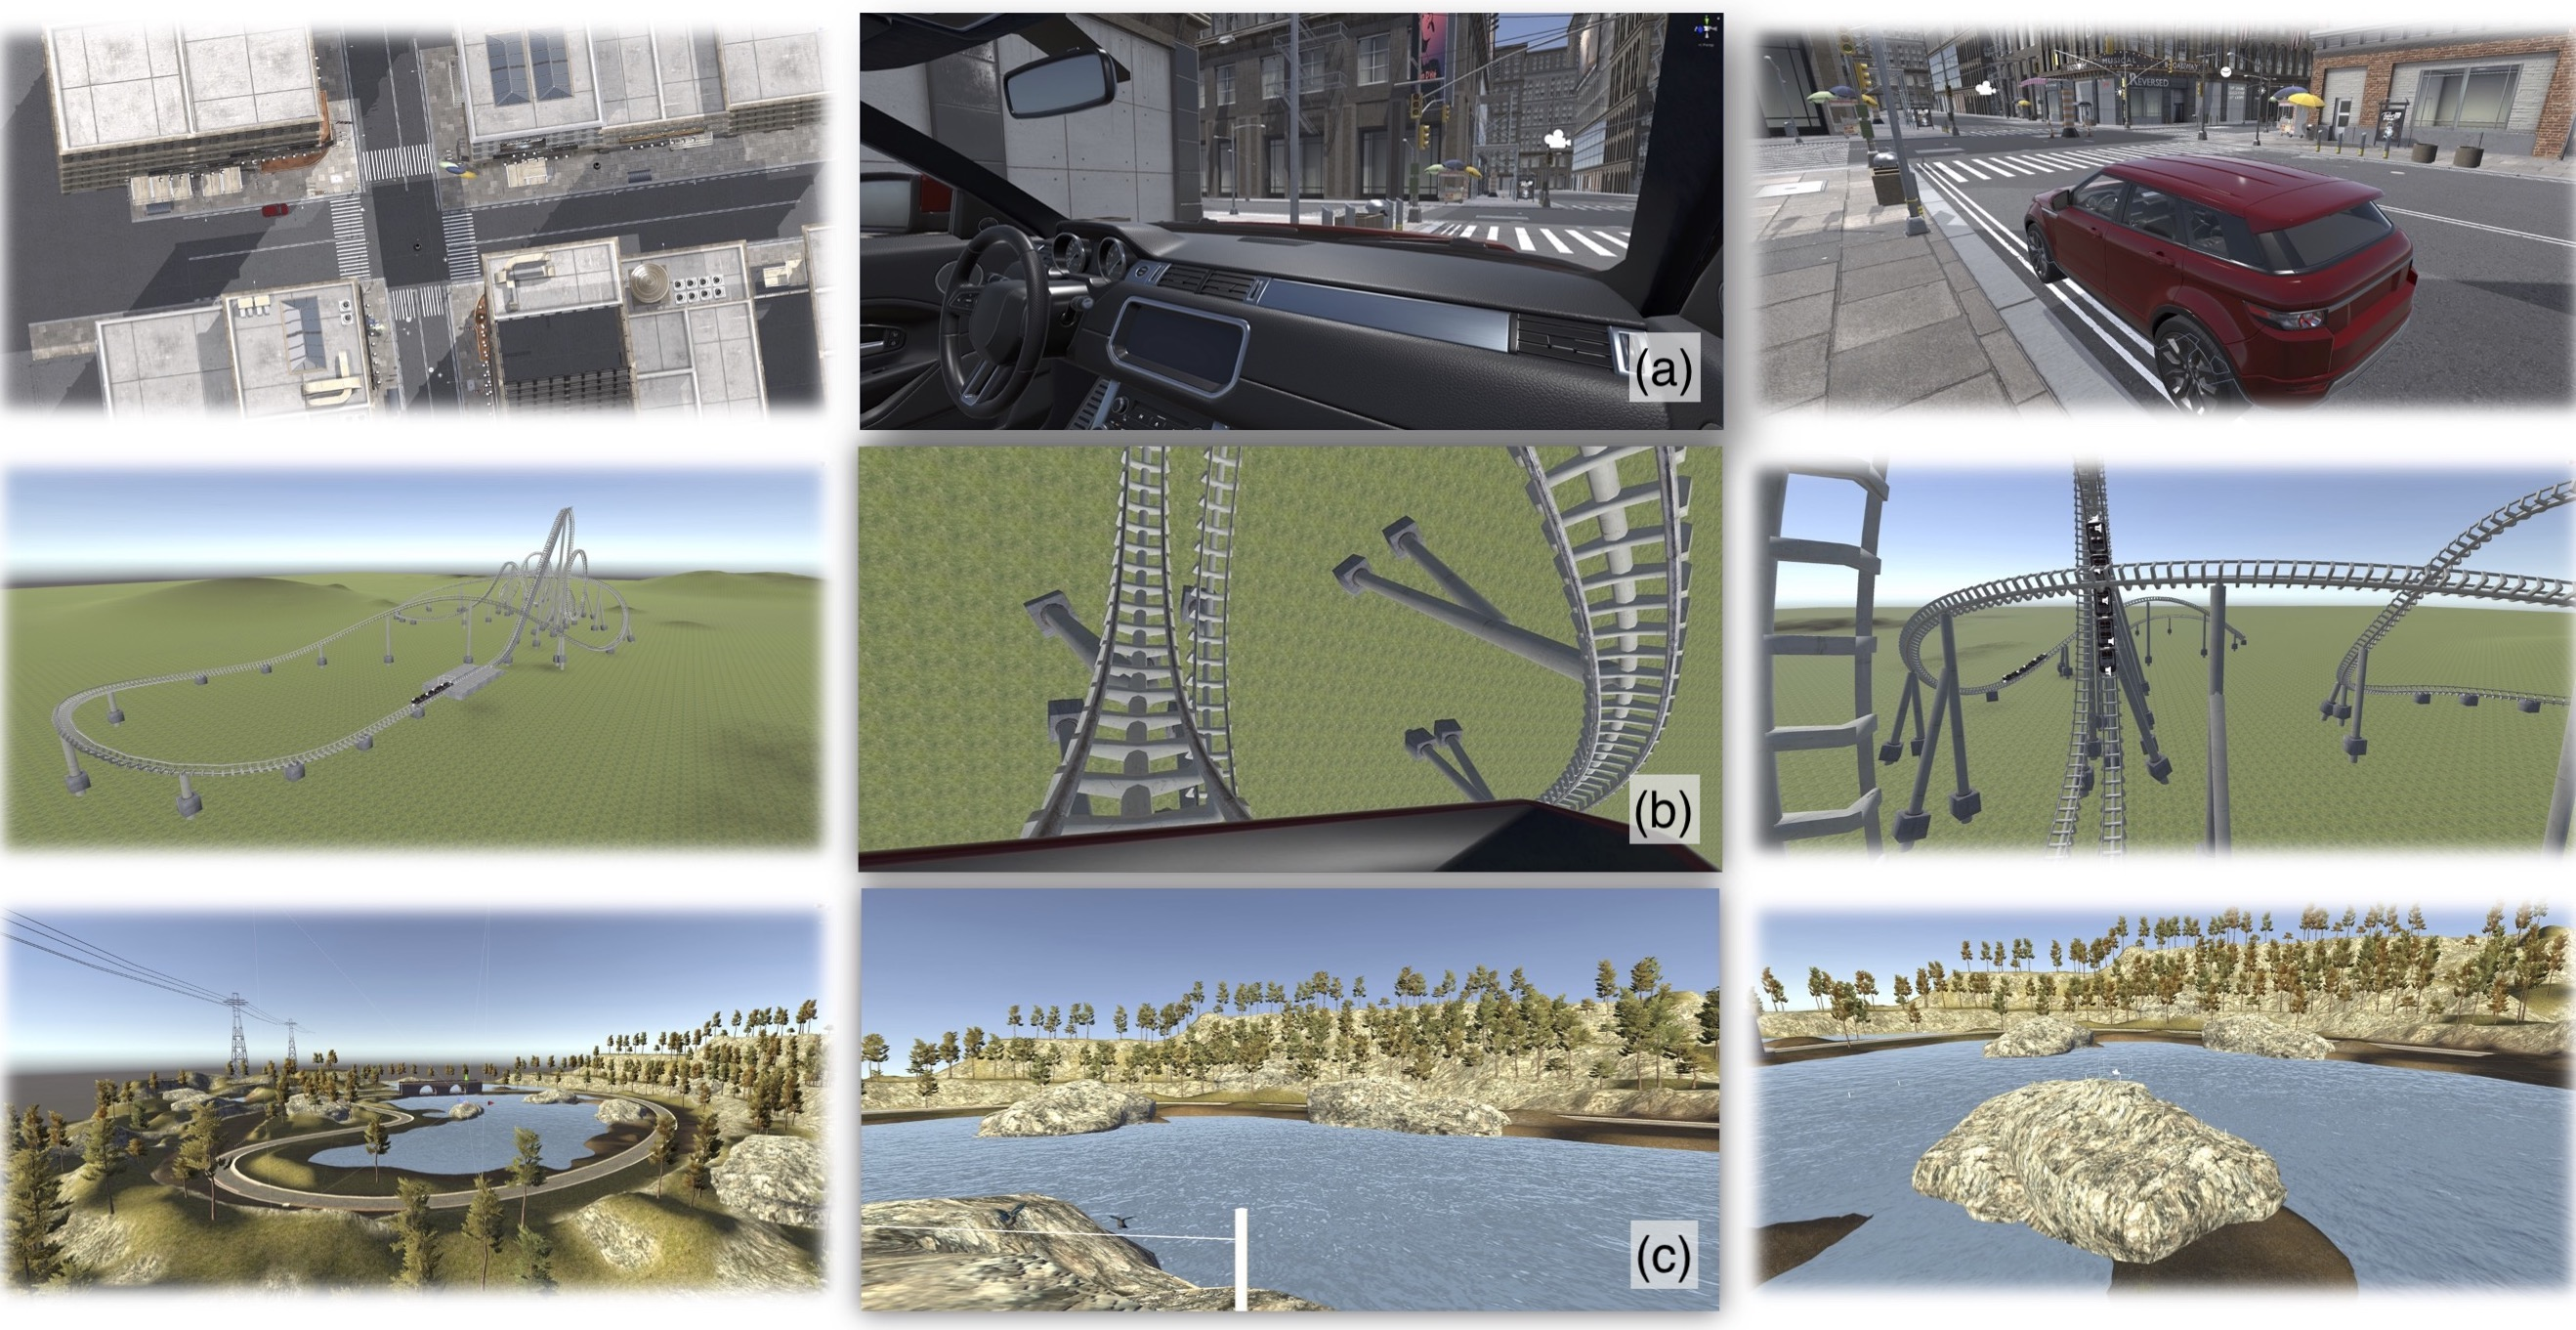
\includegraphics[width=0.9\textwidth]{Experimental_Image.jpg}
  \caption{Screenshots of three experimental scenes in virtual environment: (a) car video, (b) roller coaster video, and (c) non-sickness video. The left image shows the appearance of the experimental environment, the middle image shows the scene from the perspective of the subject, and the right image is a single shot that captures the environment around the subject.}
  \label{fig1}
\end{figure*}


\subsection{Participants}
Thirty participants (26 males and 4 females) aged between 21 and 39 years (mean age = 23.57; SD = 4.26) were recruited for the study. One participant who experienced severe CS symptoms could not complete all experimental tests. None of the participants suffered from vertigo, epilepsy, or any other condition that could be aggravated by wearing an immersive HMD. All participants had a normal naked-eye or corrected-to-normal vision with contact lenses. Written informed consent was obtained from all participants prior to the experiment. The participants could terminate the experiment at any time. The study was approved by the Research Ethics Committee of Tokyo Metropolitan University.

\subsection{Materials}
The VR headset used in this study was the HTC Vive Pro Eye with Tobii® eye-tracking technology.
The maximum sampling frequency of eye-related indices is 120 Hz. However, a flicker problem had occurred when obtaining eye-related indices at this frequency; thus, the eye-tracking frequency was reduced to 50 Hz. 
The HMD screen is a dual organic light-emitting diode screen with a resolution of 1440 × 1600 pixels per eye. The field of viewing angle is 110° with a refresh rate of 90 Hz. Audio can be played through the integrated Vive headphones. The personal computer (PC) used was equipped with an Intel Core i7-11800H CPU running at 2.30 GHz, 16 GB RAM, and an NVIDIA GeForce RTX 3070 GPU. 

As CS-inducing scenes, we selected a car video and a roller coaster video. The car video included movements such as sudden deceleration, sudden reversals, sudden acceleration, swerving, and meandering driving. A VR camera was installed in the front passenger seat of a left-hand-drive car to provide a clear view of the surrounding scenery (Fig. 1(a)). The roller coaster video included rotations and diagonal movements of the cart. A VR camera was placed on the first cart of the train, giving a user a front-line experience (Fig. 1(b)). In the other video (Fig. 1(c)), hereafter called the non-sickness video, a user was “seated” beside a quiet lake, which was intended to induce a calm, relaxed sensation. No sickness-reducing technology was applied to these VR videos. All experiments were conducted through Steam VR and Unity 3D, and eye-related indices were collected using the VIVE Eye and Facial Tracking SDK (SRanipal SDK) provided by HTC.

\subsection{Procedure}
In this experiment, we presented two conditions. Each condition involved only one of the sickness videos (either car or roller coaster video) to induce CS in the participants. We deemed it unethical to have participants view both sickness videos in a single condition. For transparency and consistency, all participants experienced both conditions, which consisted of the following sequences:

\begin{itemize}
    \item Condition 1: Non-sickness video → Car video → Non-sickness video
    \item Condition 2: Non-sickness video → Roller coaster video → Non-sickness video
\end{itemize}

As illustrated in Fig. 2, each sickness video was preceded and followed by a non-sickness video. The sickness videos were approximately 5-min long, while the non-sickness video was 1-min long. Participants sat on a chair and viewed a combination of the prepared videos. After viewing one set of scenes, they were allowed to rest until their CS symptoms subsided before experiencing the other condition (Fig. 2). To reduce the order effect, the two conditions were presented in a counterbalanced way across the participants.

In all videos, the participants could freely change their field-of-view. 
Eye tracking was also calibrated before the start of the experiment.
During the video experience, the participants subjectively indicated one of the four levels of CS severity by placing their thumb at the appropriate position on the trackpad of the HTC Vive controller (2018), as depicted in Fig. 3. The trackpad is equipped with a sensor that allows continuous recording by simply placing a finger on it (no forceful pushing or clicking was required). Analogous to the SSQ crafted as a subjective assessment tool for simulator sickness, we assessed four degrees of CS severity: None, Slight, Moderate, and Severe. Data on CS severity were recorded continuously at a sampling rate of 50 Hz. Each participant completed the entire experiment in approximately 1 h.

 \begin{figure}[th]
  \begin{center}
    \includegraphics*[width=1.0\linewidth]{Procedure.png}
  \end{center}
  % \vspace*{-6mm}
  \caption{Procedure of the user data measurement.}
  \label{figure}
\end{figure}

 \begin{figure}[th]
  \begin{center}
    \includegraphics*[width=0.7\linewidth]{Evaluation.png}
  \end{center}
  % \vspace*{6mm}
  \caption{Illustration of the coordinate-segmentation method using the HTC Vive controller trackpad for 4-level CS evaluation.}
  \label{figure}
\end{figure}

\subsection{Eye-Related Indices}

\begin{figure*}[h!]
  \centering
  
\includegraphics[width=0.9\textwidth]{Eye_HMD.jpg}
  \caption{(Left) Coordinate system of HTC Vive Pro Eye, and (right) a diagram showing gaze origin position and normalized gaze direction vector.}
  \label{figure}
\end{figure*}

As part of this study, we examined various eye-related indices to assess their potential as indicators for gauging the severity of CS. Among these indices, pupil diameter emerged as a notable candidate. Fluctuations in pupil diameter are widely recognized to be influenced by a range of factors, including emotional states \cite{Bradley_2008, Tarnowski_2020}, and fatigue \cite{Wang_2017}—conditions frequently associated with CS experiences \cite{Kaufeld_2022, Kim_2_2021, LaViola_2020}. Therefore, variations in pupil diameter provide significant insights in this context. Nonetheless, we have taken into consideration that pupil diameter constitutes just among several contributing factors. Our approach comprehensively integrates an array of eye-related indices to aptly predict the severity of CS.
We collected a total of 11 features from five types of eye-related indices as follows: 

\begin{itemize}
    \item Normalized pupil positions of both eyes (four features of $x$ and $y$ axes for both eyes)
    \item Pupil diameters of both eyes [mm] (two features)
    \item Gaze deviation from the center of the screen (one feature)
    \item Angular velocity of eye gaze at 0.02-s intervals [deg/s] (one feature)
    \item Gaze origin position [mm] (three features of $x$, $y$, and $z$ axes)
\end{itemize}

As shown in Fig. 4 (right), the gaze deviation from the center of screen $d_{xy}$ is defined in the HTC Vive Pro Eye coordinate system utilizing the $x$-direction gaze vector $x_b$, the $y$-direction gaze vector $y_b$, and the center of screen coordinates ($x_o$, $y_o$) = (0,0):
\begin{align}
    d_{xy}=\sqrt{(x_b-x_o)^2+(y_b-y_o)^2}
\end{align}
The center of screen coordinates refers to the system origin situated at the center of the two lenses of the HMD (Fig. 4), while the gaze origin position represents the central coordinate of the straight line connecting the central coordinates of both corneas (Fig. 4 (right)). 
The pupil positions of both eyes and the gaze direction vector are automatically provided as normalized values according to the HTC Vive Pro Eye specifications. All data were recorded in the right-handed coordinate system (Fig. 4 (left)). 

These eye-related indices were then individually normalized using the following equation for subsequent DL applications:
\begin{align}
    x_i^{norm} = \dfrac{x_i^{raw} - \mu}{\sigma}
\label{eq_norm}
\end{align}
Here, $x$ represents time-series data, $\mu$ represents the mean of $x$, $\sigma$ represents the standard deviation of $x$, $x_i^{raw}$ represents the $i_{th}$ data point of $x$, and $x_i^{norm}$ represents the data after normalization. We adopted the methodology of individual normalization and integrated learning processes that accommodate temporal characteristics. This approach was used to alleviate the influence of static factors such as gender and age on eye-related indices \cite{Cantoni_2020}. The process of normalization has enabled us to mitigate these effects and regard them as inherent noise within the measured data. A noteworthy and pragmatic advantage of this methodology is its ability to obviate the necessity for distinguishing among VR participants, thereby simplifying the implementation process. 

Furthermore, missing intervals in eye-related indices due to factors such as blinking were interpolated using a linear interpolation method based on data with and without missing values. Overall, we obtained approximately 42,000 data points for each participant who completed the experiment, comprising eye-related indices and CS severity data based on a sampling rate of 50 Hz for the full VR viewing time of 14 min per participant.


\section{Deep Learning Model}%%%%%%%%%%%%%%%%%%%%
In this study, we aimed to achieve highly accurate prediction of CS occurrence and severity utilizing the attention-based long short-term memory fully convolutional network (ALSTM-FCN)-based DL model proposed by Karim et al. \cite{Karim_2017}. The ALSTM-FCN model is a variation of the LSTM-FCN model that incorporates an attention mechanism. Besides, classification methods based on FCN and LSTM-FCN models are more accurate than conventional methods \cite{Wang_DL_2016, Karim_2017}.


\subsection{Temporal Convolutional Networks (TCN)}
We extracted eye-related indices as features using temporal convolutional networks (TCNs) in FCNs. A TCN is a CNN variant for sequence modeling that uses time-series data as input. As stated in Lea et al. \cite{Lea_2016}, let $X_t \in \mathbb{R}^{F_0}$ be the input feature vector of length $F_0$ in time step $t$ for $1  \leq t \leq T$. Each sequence may have a specific time $T$, and the number of time steps in each layer $l$ is denoted as $T_l$. The true label for each frame is given by $y_t \in \{1, . . . , C\}$, where $C$ represents the number of classes. 

For each convolutional layer, we applied a set of one-dimensional filters that capture changes in input signals. The filters for each layer $l$ are parameterized by tensor $W^{(l)} \in \mathbb{R}^{F_l \times d \times F_{l-1}}$ and biases $b^{l} \in \mathbb{R}^{F_l}$, where $d$ represents the filter duration. In the same layer, the $i_{th}$ component of the unnormalized activation $\widehat{E}_t^{(l)} \in \mathbb{R}^{F_l}$ is a function of the incoming normalized activation matrix $E^{(l-1)} \in \mathbb{R}^{F_{l-1} \times T_{l-1}}$ from the previous layer \cite{Lea_2016}
\begin{align}
    \widehat{E}_{i,t}^{(l)} = f \Biggl(b_i^{(l)} + \sum_{t'=1}^d \Bigr \langle W_{i,t',.}^{(l)}, E_{.t+d-t'}^{(l-1)} \Bigr \rangle \Biggl)
\end{align}
for each time $t$, where $f(\cdot)$ denotes the rectified linear unit (ReLU) function.

A basic convolution block consists of a convolution layer, followed by a normalization process and the ReLU activation function. Overall, the FCN model is composed of three convolutional blocks and a global average pooling (GAP) layer \cite{Lin_2013} applied after the final convolutional block.

\subsection{Long Short-term Memory (LSTM)}

\begin{figure}[h]
    \includegraphics*[width=\linewidth]{LSTM.jpg}
    \caption{Schematic of the internal structure of the LSTM unit.}
    \label{figure}
\end{figure}

LSTM is a type of recurrent neural network (RNN) architecture designed to handle the problem of vanishing gradients in traditional RNNs \cite{Hochreiter_1997}. LSTM has an internal memory cell that can retain information for longer periods, allowing the network to better handle time-dependent sequences. Fig. 5 shows a schematic of the LSTM unit. The LSTM unit is composed of three gates and a memory cell to store long-term information: which input gate $i_t$, forget gate $f_t$, output gate $o_t$, and memory cell $c_t$, respectively. The calculation process of LSTM is outlined below. Here, $x$ represents the input to the unit, $h$ represents the output of the unit, $b$ represents the biases, $W$ represents the weights, and $\odot$ denotes the element-wise product. In addition, the subscripts of weights ($W$) and biases ($b$) indicate which weight or bias is by the first and second letters.

The input gate $i_t$ and the input data $g_t$ are calculated using two activation functions ($\sigma$: sigmoid function; $tanh$: hyperbolic tangent function), as expressed in Eqs. (4) and (5). 

\begin{align}
    i_t = \sigma(W_{xi}x_t + b_{xi} + W_{hi}h_{t-1} + b_{hi})
\end{align}
\begin{align}
    g_t = tanh(W_{xg}x_{t} + W_{hg}h_{t-1} + b_g)
\end{align}
The forget gate $f_t$ decides which information to preserve and which to discard, and it is controlled by the sigmoid function, as expressed in Eq. (6).
\begin{align}
    f_t = \sigma(W_{xf}x_t + b_{xf} + W_{hf}h_{t-1} + b_{hf})
\end{align}
The state of the memory cell $c_t$ at time step t is given by Eq. (7), and it is the sum of the input gate $i_t$ multiplied by the input data $g_t$ and the forget gate $f_t$ multiplied by the state of the memory cell $c_{t-1}$ from the previous time step.
\begin{align}
    c_t = f_t \odot c_{t-1} + i_t \odot g_t
\end{align}
The output gate $o_t$ and the output $h_t$ are calculated using two activation functions, as expressed in Eqs. (8) and (9).
\begin{align}
    o_t = \sigma(W_{xo}x_t + b_{xo} + W_{ho}h_{t-1} + b_{ho})
\end{align} 
\begin{align}
    h_t = o_t \odot tanh(c_t)
\end{align}
Note that the input gate $i_t$ and input data $g_t$ of LSTM are different and that the input gate $i_t$ determines the addition of new information to the memory cell. The input gate $i_t$ is a combination of input data $x_t$ and previous output $h_{t-1}$.


\subsection{Attention Mechanism}
The attention mechanism is a DL technique for extracting important information from multiple input sequences and combining them to generate an output sequence. The attention concept was introduced by Bahdanau et al. \cite{Bahdanau_2014}.
The attention mechanism incorporates contextual information from input sequences. The output element $a_i$ is determined by a sequence of annotations ($h_1, h_2, ..., h_n$), where n represents the maximum length of an input sequence. Each annotation $h_i$ contains information about the entire input sequence, with a strong focus on parts surrounding the $i_{th}$ element of the input sequence.
$a_i$ can be calculated using Eq. (10).
\begin{align}
    a_i = \sum_{j=1}^n W_{ij}h_{j}
\end{align}
Here, $W_{ij}$ represents the weights of each annotation $h_{j}$. The attention weights are calculated using a dot product between the annotations, and the softmax function is used to normalize the results. This can be mathematically represented as follows:

\begin{align}
    W_{ij} = \frac{\exp(h_i^T h_j)}{\sum_{k=1}^{n} \exp(h_i^T h_k)}
\end{align}
Where $h_i$ and $h_j$ denote the $i_{th}$ and $j_{th}$ annotations, respectively, and T represents the transpose of the vector. 


\subsection{ALSTM-FCN model}

\begin{figure*}[t!]
  \centering
  
\includegraphics[width=0.9\textwidth]{ALSTM-FCN.jpg}
  \caption{Configuration diagram of ALSTM-FCN model used in the experiment}
  \label{ALSTM-FCN}
\end{figure*}

The architecture of the ALSTM-FCN model consists of two parts: an LSTM network with an attention mechanism and an FCN, as discussed in previous sub-subsections. The ALSTM-FCN model used in this study is depicted in Fig. 6.

The model has two LSTM layers stacked on top of each other. The first LSTM layer has 256 units and is followed by a “Layer Normalization (LN)” layer \cite{Ba_2016}, which normalizes the output of the LSTM layer. The output of this layer is passed to a Dropout layer with a dropout rate of 0.2. This means that during training, 20\% of the activations in the output of the first LSTM layer will be set to zero. This is done to prevent overfitting by randomly dropping out some activations. The model is forced to learn multiple independent representations of the same input, enhancing the robustness of the model to unseen data. The second LSTM layer has 128 units, followed by a LN layer, an Attention layer, and a Dropout layer with a dropout rate of 0.2. The Attention layer is used to weigh the importance of each timestep in the LSTM output and generate a weighted sum of the LSTM output. 

Similarly, FCN layers are also defined. The FCN layers are defined using a series of one-dimensional convolutional (Conv1D) layers. The first Conv1D layer has 128 filters of size 8, the second Conv1D layer has 256 filters of size 5, and the third Conv1D layer has 128 filters of size 3. Each Conv1D layer is followed by a LN layer and an activation layer with the ReLU activation function. This function is used to introduce nonlinearity into the model and allow the model to learn more complex representations of the data. The output of the last Conv1D layer is passed through a one-dimensional GAP layer. This layer takes the average of the values of the last Conv1D layer along the temporal axis. This is used to reduce the number of parameters in the model and to make the model more robust to variations in input sequences. 

The output of the LSTM and FCN layers are concatenated and passed through a Dense layer with the softmax activation. The Dense layer has the same number of units as the number of classes in the output. The final output is a probability distribution over the classes.




\section{Cybersickness Prediction Using Deep Learning}

\subsection{Evaluation Methods}
In this analysis, we conducted two evaluations to verify the feasibility of high-frequency CS prediction: 
\begin{itemize}
    \item Five-fold cross-validation using all data obtained from all subjects.
    \item Five-fold cross-validation on individual data, repeated for all subjects.
\end{itemize}
The k-fold cross-validation is a method for evaluating the performance of ML models. It involves dividing a dataset into k equally sized folds, training the model on k-1 of the folds, and evaluating it on the remaining one. This process is repeated k times, with each fold serving as the test set once. This method helps reduce the variance in model performance estimates and provides a better understanding of how the model will perform on unseen data \cite{Bengio_2004}.
The cross-validation using all data was conducted to verify the feasibility of high-frequency CS prediction with a high generalization ability suitable for all data. The cross-validation experiment on individual data was conducted to develop individual learning models and verify the feasibility of high-frequency CS prediction suitable for each individual. 

The ALSTM-FCN model was used as the training model. For comparison purposes, a simple LSTM (sLSTM) model (with 128 units), the FCN model (only the FCN part of ALSTM-FCN), and the LSTM-FCN model (the same model as ALSTM-FCN without the Attention layer) were also used. We used $n$-second ($n$ = 1, 5, and 10) time-series eye-related indices as features for each learning. 
To the best of our knowledge, no study has verified the possibility of predicting CS faster than the prediction interval of 30 s by Islam et al. using eye-related indices \cite{Islam_2021}. The ground truth label was based on the evaluation of CS recorded 0.5 s after the last time-series eye-related indices for each $n$ [s]. This time value considers the delay in evaluating the CS of a subject, as demonstrated by Nalivaiko et al. \cite{Nalivaiko_2015}.

In this analysis, we performed a 4-level severity classification task for CS prediction, with the categories being 0 (none), 1 (slight), 2 (moderate), and 3 (severe), as well as a binary classification task for CS occurrence, dividing into the non-sickness group (0 and 1) and sickness group (2 and 3). The accuracy, precision, and recall metrics were used to evaluate the obtained DL models calculated from the following equations and confusion matrix (Fig. 7):


\begin{align}
    accuracy = \frac{T_P + F_N}{T_P + T_N + F_P + F_N} \\
    precision = \frac{T_P}{T_P + F_P} \\
    recall = \frac{T_P}{T_P + F_N}
\end{align}

\begin{figure}[th]
  \begin{center}
    \includegraphics*[width=0.7\linewidth]{Precision_Recall.png}
  \end{center}
  \caption{Confusion matrix of predicted labels and actual labels}
  \label{figure}
\end{figure}

\subsection{Hyperparameter and Loss Function}
The number of units for the two LSTM layers was determined through hyperparameter tuning using data from all subjects, whereas the parameters for the Conv1D layers were configured in accordance with the model proposed by Karim et al. \cite{Karim_2017}. To counteract overfitting, early stopping was implemented with a patience value of 10 during model training. The model was compiled using the Adam optimizer \cite{Kingma_2014} with 300 epochs and a batch size of 128. The Adam optimizer iteratively adjusts the parameters of the model during training to minimize the loss function, which is computed iteratively, thereby enhancing model performance. Additionally, distinct loss functions were used for the multiclass and binary classification tasks. For the multiclass classification task, categorical cross entropy was used as the loss function:
\begin{align}
    L_{categorical} = -\sum_{i=1}^{C}t_i*log(y_i)
\end{align}
In this context, $C$ denotes the overall count of classes; $t_i$ represents the true label for class $i$, presented as a one-hot encoded vector; and $y_i$ is the predicted probability for class $i$, calculated by the model. For the binary classification task, we used binary cross entropy as the loss function: 
\begin{align}
    L_{binary} = -(t * log(y) + (1 - t) * log(1 - y))
\end{align}
where $t$ represents the true label, and $y$ denotes the predicted probability for the positive class.

\subsection{Evaluation of Models for All Subjects}


\begin{table*}[htbp!]
\caption{Results from a 4-level classification of CS severity through a five-fold cross-validation approach, using data from all participants. The “$n$-value” denotes the duration in seconds of the time-series data used as features.}
\label{tab:my-table}
\centering

\begin{tabular*}{0.9\textwidth}{c|c|c|cccc|cccc}
\hline
  \multirow{2}{*}{\textbf{n-value}} &
  \multirow{2}{*}{\textbf{Model}} &
  \multirow{2}{*}{\textbf{Accuracy}} &
  \multicolumn{4}{c|}{\textbf{Precision}} &
  \multicolumn{4}{c}{\textbf{Recall}} \\ \cline{4-11} 
 &
   &
   &
  \multicolumn{1}{c|}{\begin{tabular}[c]{@{}c@{}}0\\    \\ (None)\end{tabular}} &
  \multicolumn{1}{c|}{\begin{tabular}[c]{@{}c@{}}1\\    \\ (Slight)\end{tabular}} &
  \multicolumn{1}{c|}{\begin{tabular}[c]{@{}c@{}}2\\    \\ (medium)\end{tabular}} &
  \begin{tabular}[c]{@{}c@{}}3\\    \\ (Severe)\end{tabular} &
  \multicolumn{1}{c|}{\begin{tabular}[c]{@{}c@{}}0\\    \\ (None)\end{tabular}} &
  \multicolumn{1}{c|}{\begin{tabular}[c]{@{}c@{}}1\\    \\ (Slight)\end{tabular}} &
  \multicolumn{1}{c|}{\begin{tabular}[c]{@{}c@{}}2\\    \\ (medium)\end{tabular}} &
  \begin{tabular}[c]{@{}c@{}}3\\    \\ (Severe)\end{tabular} \\ \hline
\multirow{4}{*}{1   [s]} &
  ALSTM-FCN &
  0.7109 &
  \multicolumn{1}{c|}{0.8175} &
  \multicolumn{1}{c|}{0.5634} &
  \multicolumn{1}{c|}{0.5920} &
  0.5764 &
  \multicolumn{1}{c|}{0.8821} &
  \multicolumn{1}{c|}{0.5243} &
  \multicolumn{1}{c|}{0.5372} &
  0.5019 \\ \cline{2-11} 
 &
  LSTM-FCN &
  0.6850 &
  \multicolumn{1}{c|}{0.8063} &
  \multicolumn{1}{c|}{0.5368} &
  \multicolumn{1}{c|}{0.5340} &
  0.4714 &
  \multicolumn{1}{c|}{0.8767} &
  \multicolumn{1}{c|}{0.5062} &
  \multicolumn{1}{c|}{0.4628} &
  0.4068 \\ \cline{2-11} 
 &
  sLSTM &
  0.6806 &
  \multicolumn{1}{c|}{0.8139} &
  \multicolumn{1}{c|}{0.5057} &
  \multicolumn{1}{c|}{0.5512} &
  0.5391 &
  \multicolumn{1}{c|}{0.8429} &
  \multicolumn{1}{c|}{0.5047} &
  \multicolumn{1}{c|}{0.5169} &
  0.4733 \\ \cline{2-11} 
 &
  FCN &
  0.5899 &
  \multicolumn{1}{c|}{0.7973} &
  \multicolumn{1}{c|}{0.4629} &
  \multicolumn{1}{c|}{0.3584} &
  0.3094 &
  \multicolumn{1}{c|}{0.7478} &
  \multicolumn{1}{c|}{0.3616} &
  \multicolumn{1}{c|}{0.5624} &
  0.2624 \\ \hline
\multirow{4}{*}{5   [s]} &
  ALSTM-FCN &
  0.6873 &
  \multicolumn{1}{c|}{0.8008} &
  \multicolumn{1}{c|}{0.5364} &
  \multicolumn{1}{c|}{0.5282} &
  0.5731 &
  \multicolumn{1}{c|}{0.8845} &
  \multicolumn{1}{c|}{0.4327} &
  \multicolumn{1}{c|}{0.5803} &
  0.3698 \\ \cline{2-11} 
 &
  LSTM-FCN &
  0.6662 &
  \multicolumn{1}{c|}{0.7801} &
  \multicolumn{1}{c|}{0.5052} &
  \multicolumn{1}{c|}{0.5433} &
  0.4729 &
  \multicolumn{1}{c|}{0.8608} &
  \multicolumn{1}{c|}{0.4635} &
  \multicolumn{1}{c|}{0.4859} &
  0.3623 \\ \cline{2-11} 
 &
  sLSTM &
  0.6720 &
  \multicolumn{1}{c|}{0.8108} &
  \multicolumn{1}{c|}{0.4841} &
  \multicolumn{1}{c|}{0.5543} &
  0.5043 &
  \multicolumn{1}{c|}{0.8332} &
  \multicolumn{1}{c|}{0.4821} &
  \multicolumn{1}{c|}{0.5344} &
  0.4462 \\ \cline{2-11} 
 &
  FCN &
  0.5648 &
  \multicolumn{1}{c|}{0.6188} &
  \multicolumn{1}{c|}{0.3862} &
  \multicolumn{1}{c|}{0.4169} &
  0.3827 &
  \multicolumn{1}{c|}{0.8903} &
  \multicolumn{1}{c|}{0.1111} &
  \multicolumn{1}{c|}{0.3388} &
  0.2385 \\ \hline
\multirow{4}{*}{10 [s]} &
  ALSTM-FCN &
  0.6754 &
  \multicolumn{1}{c|}{0.7978} &
  \multicolumn{1}{c|}{0.5367} &
  \multicolumn{1}{c|}{0.4921} &
  0.5349 &
  \multicolumn{1}{c|}{0.8843} &
  \multicolumn{1}{c|}{0.3654} &
  \multicolumn{1}{c|}{0.5690} &
  0.5208 \\ \cline{2-11} 
 &
  LSTM-FCN &
  0.6704 &
  \multicolumn{1}{c|}{0.7626} &
  \multicolumn{1}{c|}{0.5346} &
  \multicolumn{1}{c|}{0.5922} &
  0.4967 &
  \multicolumn{1}{c|}{0.8525} &
  \multicolumn{1}{c|}{0.4935} &
  \multicolumn{1}{c|}{0.4843} &
  0.4280 \\ \cline{2-11} 
 &
  sLSTM &
  0.6769 &
  \multicolumn{1}{c|}{0.8109} &
  \multicolumn{1}{c|}{0.5084} &
  \multicolumn{1}{c|}{0.5220} &
  0.6210 &
  \multicolumn{1}{c|}{0.8519} &
  \multicolumn{1}{c|}{0.5510} &
  \multicolumn{1}{c|}{0.4251} &
  0.4753 \\ \cline{2-11} 
 &
  FCN &
  0.5648 &
  \multicolumn{1}{c|}{0.6459} &
  \multicolumn{1}{c|}{0.4110} &
  \multicolumn{1}{c|}{0.3797} &
  0.4918 &
  \multicolumn{1}{c|}{0.8442} &
  \multicolumn{1}{c|}{0.3059} &
  \multicolumn{1}{c|}{0.2685} &
  0.1852 \\ \hline
\end{tabular*}
\end{table*}


\begin{table*}[htbp!]
\caption{Results from a binary classification of CS occurrence through a five-fold cross-validation approach, using data from all participants. The “$n$-value” denotes the duration in seconds of the time-series data used as features.}
\label{tab:my-table}
\centering
\begin{tabular*}{0.68\textwidth}{c|c|c|cc|cc}
\hline
\multirow{2}{*}{\textbf{n-value}} &
  \multirow{2}{*}{\textbf{Model}} &
  \multirow{2}{*}{\textbf{Accuracy}} &
  \multicolumn{2}{c|}{\textbf{Precision}} &
  \multicolumn{2}{c}{\textbf{Recall}}\\ \cline{4-7} 
                            &           &        & \multicolumn{1}{c|}{Non-Sickness} & Sickness & \multicolumn{1}{c|}{Non-Sickness} & Sickness \\ \hline
\multirow{4}{*}{1   [s]}  & ALSTM-FCN & 0.8253 & \multicolumn{1}{c|}{0.8828}       & 0.6247   & \multicolumn{1}{c|}{0.8915}       & 0.6041   \\ \cline{2-7} 
                            & LSTM-FCN  & 0.8287 & \multicolumn{1}{c|}{0.8733}       & 0.6483   & \multicolumn{1}{c|}{0.9094}       & 0.5588   \\ \cline{2-7} 
                            & sLSTM      & 0.8282 & \multicolumn{1}{c|}{0.8772}       & 0.6407   & \multicolumn{1}{c|}{0.9032}       & 0.5773   \\ \cline{2-7} 
                            & FCN       & 0.7929 & \multicolumn{1}{c|}{0.8408}       & 0.5693   & \multicolumn{1}{c|}{0.9012}       & 0.4334   \\ \hline
\multirow{4}{*}{5   [s]}  & ALSTM-FCN & 0.8357 & \multicolumn{1}{c|}{0.8754}       & 0.6793   & \multicolumn{1}{c|}{0.9150}       & 0.5801   \\ \cline{2-7} 
                            & LSTM-FCN  & 0.8125 & \multicolumn{1}{c|}{0.8260}       & 0.7058   & \multicolumn{1}{c|}{0.9568}       & 0.3395   \\ \cline{2-7} 
                            & sLSTM      & 0.8194 & \multicolumn{1}{c|}{0.8723}       & 0.6286   & \multicolumn{1}{c|}{0.8936}       & 0.5801   \\ \cline{2-7} 
                            & FCN       & 0.8019 & \multicolumn{1}{c|}{0.8253}       & 0.6408   & \multicolumn{1}{c|}{0.9405}       & 0.3477   \\ \hline
\multirow{4}{*}{10   [s]} & ALSTM-FCN & 0.8212 & \multicolumn{1}{c|}{0.8337}       & 0.7298   & \multicolumn{1}{c|}{0.9575}       & 0.3755   \\ \cline{2-7} 
                            & LSTM-FCN  & 0.7949 & \multicolumn{1}{c|}{0.8125}       & 0.6518   & \multicolumn{1}{c|}{0.9501}       & 0.2988   \\ \cline{2-7} 
                            & sLSTM      & 0.8260 & \multicolumn{1}{c|}{0.8686}       & 0.6527   & \multicolumn{1}{c|}{0.9105}       & 0.5498   \\ \cline{2-7} 
                            & FCN       & 0.7828 & \multicolumn{1}{c|}{0.7986}       & 0.6154   & \multicolumn{1}{c|}{0.9566}       & 0.2233   \\ \hline
\end{tabular*}
\end{table*}







\begin{figure*}[htbp!]
    \centering
    \subfloat[]{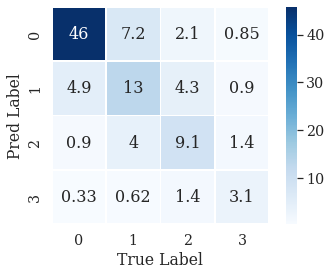
\includegraphics[width=40mm]{CM_Image/All/4class/ALSTM-FCN/1.png}\label{fig:ALSTM-FCN-1}}
    \hfill
    \subfloat[]{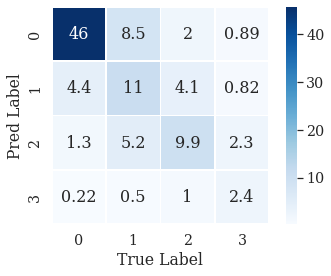
\includegraphics[width=40mm]{CM_Image/All/4class/ALSTM-FCN/5.png}\label{fig:ALSTM-FCN-5}}
    \hfill
    \subfloat[]{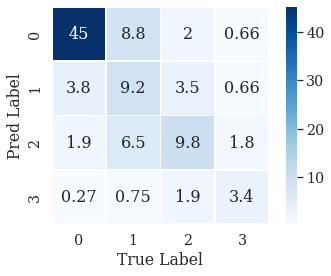
\includegraphics[width=40mm]{CM_Image/All/4class/ALSTM-FCN/10.png}\label{fig:ALSTM-FCN-10}}
    \caption{Illustration of the confusion matrix of the 4-level classification of CS severity, established through a five-fold cross-validation approach using the ALSTM-FCN model. The analysis is conducted using data from all participants (\%). Subcaptions denoting the duration in seconds of the time-series data used as features are as follows: (a) 1 [s], (b) 5 [s], (c) 10 [s].}
    \label{fig:ALSTM-FCN}
\end{figure*}


\begin{figure*}[htbp!]
    \centering
    \subfloat[]{
    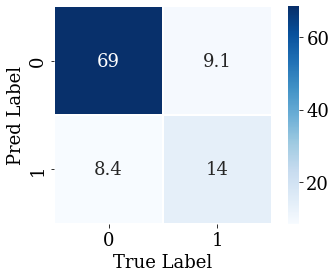
\includegraphics[width=40mm]{CM_Image/All/2class/ALSTM-FCN/1.png}
    \label{fig:2class-1s}
    }
    \hfill
    \subfloat[]{
    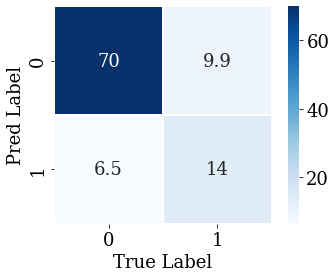
\includegraphics[width=40mm]{CM_Image/All/2class/ALSTM-FCN/5.png}
    \label{fig:2class-5s}
    }
    \hfill
    \subfloat[]{
    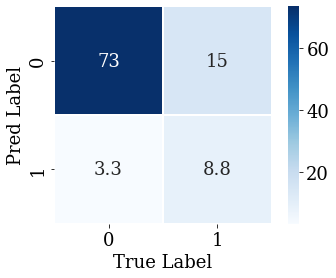
\includegraphics[width=40mm]{CM_Image/All/2class/ALSTM-FCN/10.png}
    \label{fig:2class-10s}
    }
    \caption{Illustration of the confusion matrix of the binary classification of CS occurrence, established through a five-fold cross-validation approach using the ALSTM-FCN model. The analysis is conducted using data from all participants (\%). Subcaptions denoting the duration in seconds of the time-series data used as features are as follows: (a) 1 [s], (b) 5 [s], (c) 10 [s].}
    \label{fig:2class}
\end{figure*}

In this section, the results of five-fold cross-validation using all data obtained from 27 of the 30 participants in the experiment are presented. The data from three participants were excluded: the data of two participants could not be obtained due to PC issues; one participant retired from the experiment and could not complete it. We conducted two classification tasks for CS: 4-level classification for the severity of CS, and binary classification for the occurrence of CS. 

For the 4-level classification task, the accuracy, precision, and recall values of the four models (ALSTM-FCN, LSTM-FCN, sLSTM, and FCN) obtained from five-fold cross-validation for $n$-second time-series eye-related indices are summarized in Table 1. The confusion matrix between predicted and actual labels using the ALSTM-FCN model is shown in Fig. 8. The ALSTM-FCN model achieved an accuracy of 71.09\% when using 1-second time-series eye-related indices as features, with high precision (81.75\%) and recall (88.21\%) values for CS severity of 0 (none). However, this model struggled to distinguish between severity levels 1 (slight), 2 (moderate), and 3 (severe).

For the binary classification task, the accuracy, precision, and recall values of the four models obtained from five-fold cross-validation for $n$-second time-series eye-related indices are summarized in Table 2. The confusion matrix between predicted and actual labels using the ALSTM-FCN model is depicted in Fig. 9. 
In the case of the ALSTM-FCN and sLSTM model, an accuracy of approximately 82\% was achieved, regardless of the value of $n$ used. 
However, the precision and recall values for the sickness group are lower than those for the non-sickness group, with a difference of up to 58.2\% in recall values observed when using the ALSTM-FCN model with an $n$-value of 10.

\subsection{Evaluation of Models for Each Subject}

\begin{table*}[htbp!]
\caption{Results from a 4-level classification analysis of CS severity, established through a five-fold cross-validation methodology for each individual participant. The “$n$-value” denotes the duration in seconds of the time-series data used as features.}
\label{tab:my-table}
\centering
\begin{tabular*}{0.9\textwidth}{c|c|c|cccc|cccc}
\hline
\multirow{2}{*}{\textbf{n-value}} &
  \multirow{2}{*}{\textbf{Model}} &
  \multirow{2}{*}{\textbf{Accuracy}} &
  \multicolumn{4}{c|}{\textbf{Precision}} &
  \multicolumn{4}{c}{\textbf{Recall}} \\ \cline{4-11} 
 &
   &
   &
  \multicolumn{1}{c|}{\begin{tabular}[c]{@{}c@{}}0\\    \\ (None)\end{tabular}} &
  \multicolumn{1}{c|}{\begin{tabular}[c]{@{}c@{}}1\\    \\ (Slight)\end{tabular}} &
  \multicolumn{1}{c|}{\begin{tabular}[c]{@{}c@{}}2\\    \\ (medium)\end{tabular}} &
  \begin{tabular}[c]{@{}c@{}}3\\    \\ (Severe)\end{tabular} &
  \multicolumn{1}{c|}{\begin{tabular}[c]{@{}c@{}}0\\    \\ (None)\end{tabular}} &
  \multicolumn{1}{c|}{\begin{tabular}[c]{@{}c@{}}1\\    \\ (Slight)\end{tabular}} &
  \multicolumn{1}{c|}{\begin{tabular}[c]{@{}c@{}}2\\    \\ (medium)\end{tabular}} &
  \begin{tabular}[c]{@{}c@{}}3\\    \\ (Severe)\end{tabular} \\ \hline
\multirow{4}{*}{1   [s]} &
  ALSTM-FCN &
  0.7934 &
  \multicolumn{1}{c|}{0.8684} &
  \multicolumn{1}{c|}{0.7145} &
  \multicolumn{1}{c|}{0.7208} &
  0.7230 &
  \multicolumn{1}{c|}{0.9134} &
  \multicolumn{1}{c|}{0.6741} &
  \multicolumn{1}{c|}{0.6931} &
  0.6979 \\ \cline{2-11} 
 &
  LSTM-FCN &
  0.7225 &
  \multicolumn{1}{c|}{0.8356} &
  \multicolumn{1}{c|}{0.6160} &
  \multicolumn{1}{c|}{0.6042} &
  0.6119 &
  \multicolumn{1}{c|}{0.8675} &
  \multicolumn{1}{c|}{0.5758} &
  \multicolumn{1}{c|}{0.5983} &
  0.6212 \\ \cline{2-11} 
 &
  sLSTM &
  0.7084 &
  \multicolumn{1}{c|}{0.8353} &
  \multicolumn{1}{c|}{0.5965} &
  \multicolumn{1}{c|}{0.5770} &
  0.5940 &
  \multicolumn{1}{c|}{0.8465} &
  \multicolumn{1}{c|}{0.5816} &
  \multicolumn{1}{c|}{0.5762} &
  0.5985 \\ \cline{2-11} 
 &
  FCN &
  0.6358 &
  \multicolumn{1}{c|}{0.7451} &
  \multicolumn{1}{c|}{0.5329} &
  \multicolumn{1}{c|}{0.4938} &
  0.5057 &
  \multicolumn{1}{c|}{0.8169} &
  \multicolumn{1}{c|}{0.4818} &
  \multicolumn{1}{c|}{0.4391} &
  0.5076 \\ \hline
\multirow{4}{*}{5   [s]} &
  ALSTM-FCN &
  0.8116 &
  \multicolumn{1}{c|}{0.8779} &
  \multicolumn{1}{c|}{0.7413} &
  \multicolumn{1}{c|}{0.7507} &
  0.7543 &
  \multicolumn{1}{c|}{0.9227} &
  \multicolumn{1}{c|}{0.6989} &
  \multicolumn{1}{c|}{0.7255} &
  0.7302 \\ \cline{2-11} 
 &
  LSTM-FCN &
  0.7228 &
  \multicolumn{1}{c|}{0.8372} &
  \multicolumn{1}{c|}{0.6142} &
  \multicolumn{1}{c|}{0.6103} &
  0.6260 &
  \multicolumn{1}{c|}{0.8611} &
  \multicolumn{1}{c|}{0.5878} &
  \multicolumn{1}{c|}{0.6120} &
  0.6046 \\ \cline{2-11} 
 &
  sLSTM &
  0.7369 &
  \multicolumn{1}{c|}{0.8509} &
  \multicolumn{1}{c|}{0.6339} &
  \multicolumn{1}{c|}{0.6232} &
  0.6354 &
  \multicolumn{1}{c|}{0.8682} &
  \multicolumn{1}{c|}{0.6031} &
  \multicolumn{1}{c|}{0.6232} &
  0.6692 \\ \cline{2-11} 
 &
  FCN &
  0.6191 &
  \multicolumn{1}{c|}{0.7326} &
  \multicolumn{1}{c|}{0.4880} &
  \multicolumn{1}{c|}{0.5150} &
  0.4861 &
  \multicolumn{1}{c|}{0.8018} &
  \multicolumn{1}{c|}{0.4666} &
  \multicolumn{1}{c|}{0.4580} &
  0.3992 \\ \hline
\multirow{4}{*}{10   [s]} &
  ALSTM-FCN &
  0.7587 &
  \multicolumn{1}{c|}{0.8459} &
  \multicolumn{1}{c|}{0.6619} &
  \multicolumn{1}{c|}{0.6729} &
  0.7220 &
  \multicolumn{1}{c|}{0.8961} &
  \multicolumn{1}{c|}{0.6183} &
  \multicolumn{1}{c|}{0.6597} &
  0.6616 \\ \cline{2-11} 
 &
  LSTM-FCN &
  0.7426 &
  \multicolumn{1}{c|}{0.8514} &
  \multicolumn{1}{c|}{0.6322} &
  \multicolumn{1}{c|}{0.6633} &
  0.6306 &
  \multicolumn{1}{c|}{0.8735} &
  \multicolumn{1}{c|}{0.6183} &
  \multicolumn{1}{c|}{0.6373} &
  0.6426 \\ \cline{2-11} 
 &
  sLSTM &
  0.7334 &
  \multicolumn{1}{c|}{0.8511} &
  \multicolumn{1}{c|}{0.6196} &
  \multicolumn{1}{c|}{0.6252} &
  0.6808 &
  \multicolumn{1}{c|}{0.8554} &
  \multicolumn{1}{c|}{0.6107} &
  \multicolumn{1}{c|}{0.6331} &
  0.6730 \\ \cline{2-11} 
 &
  FCN &
  0.6283 &
  \multicolumn{1}{c|}{0.7452} &
  \multicolumn{1}{c|}{0.5092} &
  \multicolumn{1}{c|}{0.5231} &
  0.4649 &
  \multicolumn{1}{c|}{0.8075} &
  \multicolumn{1}{c|}{0.4752} &
  \multicolumn{1}{c|}{0.4916} &
  0.4030 \\ \hline
\end{tabular*}
\end{table*}





\begin{table*}[htbp!]
\caption{Results from a binary classification analysis of CS occurrence, established through a five-fold cross-validation methodology for each individual participant. The “$n$-value” denotes the duration in seconds of the time-series data used as features.}
\label{tab:my-table}
\centering
\begin{tabular*}{0.68\textwidth}{c|c|c|cc|cc}
\hline
\multirow{2}{*}{\textbf{n-value}} &
  \multirow{2}{*}{\textbf{Model}} &
  \multirow{2}{*}{\textbf{Accuracy}} &
  \multicolumn{2}{c|}{\textbf{Precision}} &
  \multicolumn{2}{c}{\textbf{Recall}}\\ \cline{4-7} 
                            &           &        & \multicolumn{1}{c|}{Non-Sickness} & Sickness & \multicolumn{1}{c|}{Non-Sickness} & Sickness \\ \hline
\multirow{4}{*}{1   [s]}  & ALSTM-FCN & 0.9123 & \multicolumn{1}{c|}{0.9359}       & 0.8389   & \multicolumn{1}{c|}{0.9474}       & 0.8085   \\ \cline{2-7} 
                            & LSTM-FCN  & 0.8801 & \multicolumn{1}{c|}{0.9134}       & 0.7760   & \multicolumn{1}{c|}{0.9272}       & 0.7414   \\ \cline{2-7} 
                            & sLSTM      & 0.8751 & \multicolumn{1}{c|}{0.9150}       & 0.7571   & \multicolumn{1}{c|}{0.9175}       & 0.7510   \\ \cline{2-7} 
                            & FCN       & 0.8134 & \multicolumn{1}{c|}{0.8548}       & 0.6590   & \multicolumn{1}{c|}{0.9034}       & 0.5487   \\ \hline
\multirow{4}{*}{5   [s]}  & ALSTM-FCN & 0.9177 & \multicolumn{1}{c|}{0.9408}       & 0.8478   & \multicolumn{1}{c|}{0.9493}       & 0.8253   \\ \cline{2-7} 
                            & LSTM-FCN  & 0.8926 & \multicolumn{1}{c|}{0.9223}       & 0.8006   & \multicolumn{1}{c|}{0.9348}       & 0.7687   \\ \cline{2-7} 
                            & sLSTM      & 0.8809 & \multicolumn{1}{c|}{0.9202}       & 0.7656   & \multicolumn{1}{c|}{0.9202}       & 0.7656   \\ \cline{2-7} 
                            & FCN       & 0.8079 & \multicolumn{1}{c|}{0.8469}       & 0.6534   & \multicolumn{1}{c|}{0.9062}       & 0.5189   \\ \hline
\multirow{4}{*}{10   [s]} & ALSTM-FCN & 0.8967 & \multicolumn{1}{c|}{0.9218}       & 0.8183   & \multicolumn{1}{c|}{0.9408}       & 0.7697   \\ \cline{2-7} 
                            & LSTM-FCN  & 0.8895 & \multicolumn{1}{c|}{0.9242}       & 0.7902   & \multicolumn{1}{c|}{0.9266}       & 0.7845   \\ \cline{2-7} 
                            & sLSTM      & 0.8867 & \multicolumn{1}{c|}{0.9207}       & 0.7858   & \multicolumn{1}{c|}{0.9273}       & 0.7697   \\ \cline{2-7} 
                            & FCN       & 0.8093 & \multicolumn{1}{c|}{0.8467}       & 0.6632   & \multicolumn{1}{c|}{0.9074}       & 0.5261   \\ \hline
\end{tabular*}
\end{table*}


\begin{figure*}[htbp!]
    \centering
    \subfloat[]{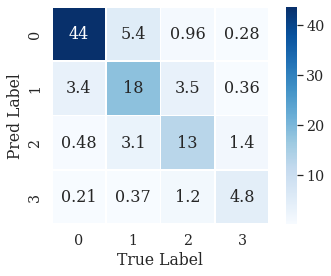
\includegraphics[width=40mm]{CM_Image/Individual/4class/ALSTM-FCN/1.png}\label{fig:ALSTM-FCN-1}}
    \hfill
    \subfloat[]{\includegraphics[width=40mm]{CM_Image/Individual/4class/ALSTM-FCN/5.png}\label{fig:ALSTM-FCN-5}}
    \hfill
    \subfloat[]{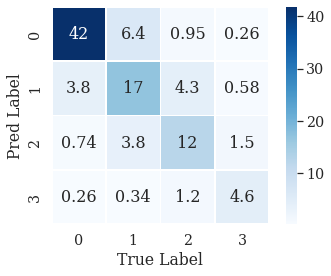
\includegraphics[width=40mm]{CM_Image/Individual/4class/ALSTM-FCN/10.png}\label{fig:ALSTM-FCN-10}}
    \caption{Illustration of the confusion matrix of the 4-level classification of CS severity, established through a five-fold cross-validation approach using the ALSTM-FCN model for each individual participant (\%). Subcaptions denoting the duration in seconds of the time-series data used as features are as follows: (a) 1 [s], (b) 5 [s], (c) 10 [s].}
    \label{fig:ALSTM-FCN}
\end{figure*}


\begin{figure*}[htbp!]
    \centering
    \subfloat[]{
    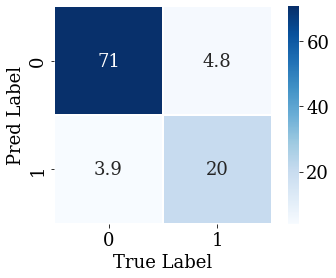
\includegraphics[width=40mm]{CM_Image/Individual/2class/ALSTM-FCN/1.png}
    \label{fig:2class-1s}
    }
    \hfill
    \subfloat[]{
    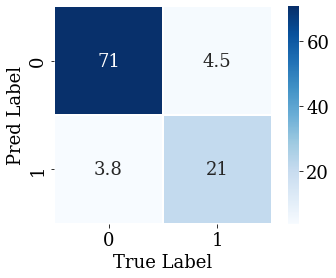
\includegraphics[width=40mm]{CM_Image/Individual/2class/ALSTM-FCN/5.png}
    \label{fig:2class-5s}
    }
    \hfill
    \subfloat[]{
    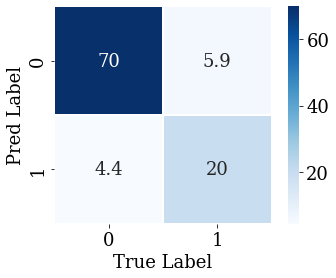
\includegraphics[width=40mm]{CM_Image/Individual/2class/ALSTM-FCN/10.png}
    \label{fig:2class-10s}
    }
    \caption{Illustration of the confusion matrix of the binary classification of CS occurrence, established through a five-fold cross-validation approach using the ALSTM-FCN model for each individual participant (\%). Subcaptions denoting the duration in seconds of the time-series data used as features are as follows: (a) 1 [s], (b) 5 [s], (c) 10 [s].}
    \label{fig:2class}
\end{figure*}


In this analysis, we conducted five-fold cross-validation on individual data to develop individual DL models and investigate whether we can perform high-frequency CS prediction suitable for each individual. The data analyzed are from 25 of the 30 participants obtained from the user study. The data from five participants were excluded: the data of two participants could not be obtained because of PC issues, one participant retired from the experiment and could not complete it, and the remaining two participants did not reach a severity level of 2 or 3 for CS throughout the experiment. This cross-validation was performed on the data of all 25 participants. We conducted two classification tasks for CS: 4-level classification for the severity of CS, and binary classification for the occurrence of CS, as described in the previous section.

For the 4-level classification task, the accuracy, precision, and recall values of the four models (ALSTM-FCN, LSTM-FCN, sLSTM, and FCN) obtained from five-fold cross-validation for $n$-second time-series eye-related indices are summarized in Table 3. The confusion matrix between predicted and actual labels using the ALSTM-FCN model is depicted in Fig. 10. The ALSTM-FCN model achieved an accuracy of 81.16\% when using 5-second time-series eye-related indices as features. 

For the binary classification task, the accuracy, precision, and recall values of the four models obtained from five-fold cross-validation for $n$-second time-series eye-related indices are summarized in Table 4. The confusion matrix between predicted and actual labels using the ALSTM-FCN model is depicted in Fig. 11. 
The maximum accuracy of the ALSTM-FCN model was above 90\%. Similarly, the non-sickness group obtained precision and recall values of over 90\%. This reveals the high classification capabilities of this model.

Overall, in both the 4-value classification and binary classification tasks, the ALSTM-FCN model outperformed the other models in terms of accuracy, precision, and recall. Moreover, the best results were achieved when 5-second time-series eye-related indices were used as features.







\section{Discussion}

\begin{table*}[h]
    \caption{Comparative analysis of CS prediction outcomes between previous studies and our proposed approach}
    \label{tab:my-table}
    \centering
    \begin{tabular*}{0.9\textwidth}{c|c|c|c|c}
    \hline
    \textbf{Reference} &
      \begin{tabular}[c]{@{}c@{}}
        \textbf{Physiological indices}\\
        \textbf{used as features}
      \end{tabular} &
      \textbf{Evaluation of CS} &
      \textbf{Learning model} &
      \textbf{Results} \\ \hline
    \begin{tabular}[c]{@{}c@{}}Kim et al. \cite{Kim_2019} \\ (2019)\end{tabular} &
      EEG &
      \begin{tabular}[c]{@{}c@{}}Original subjective evaluation\\ (after experiment, \\ not in immersive)\end{tabular} &
      \begin{tabular}[c]{@{}c@{}}CNN,\\ LSTM\end{tabular} &
      \begin{tabular}[c]{@{}c@{}}Accuracy of 89.16\%\\ in 5-level classification\end{tabular} \\ \hline
    \begin{tabular}[c]{@{}c@{}}Agundez et al. \cite{Agundez_2019} \\ (2019)\end{tabular} &
      \begin{tabular}[c]{@{}c@{}}ECG, EED, BR, \\ Skin conductivity,\\ Game parameters in VR\end{tabular} &
      \begin{tabular}[c]{@{}c@{}}SSQ\\ (after experiment, \\ not in immersive)\end{tabular} &
      \begin{tabular}[c]{@{}c@{}}SVM,\\ KNN,\\ Multilayer perceptron \end{tabular} &
      \begin{tabular}[c]{@{}c@{}}Accuracy of 82\%\\ in binary classification.\\ \\ Accuracy of 56\%\\ in ternary classification.\end{tabular} \\ \hline
    \begin{tabular}[c]{@{}c@{}}Islam et al. \cite{Islam_2_2020} \\ (2020)\end{tabular} &
      HR, BR, GSR &
      \begin{tabular}[c]{@{}c@{}}Shortened FMS collected\\  every 2 min.\\ (in immersive)\end{tabular} &
      CNN-LSTM &
      \begin{tabular}[c]{@{}c@{}}Accuracy of 97.44\% \\ in ternary classification.\end{tabular} \\ \hline
    \begin{tabular}[c]{@{}c@{}}Islam et al. \cite{Islam_2021} \\ (2021)\end{tabular} &
      Eye-related indices &
      \begin{tabular}[c]{@{}c@{}}Shortened FMS collected\\ every 30 s.\\ (in immersive)\end{tabular} &
      CNN-LSTM &
      \begin{tabular}[c]{@{}c@{}}Accuracy of 80.7\% \\ in 4-level classification.\end{tabular} \\ \hline
    \begin{tabular}[c]{@{}c@{}}Chang et al. \cite{Chang_2021} \\ (2021)\end{tabular} &
      Eye-related indices &
      \begin{tabular}[c]{@{}c@{}}SSQ\\ (after experiment, \\ not in immersive)\end{tabular} &
      Multiple regression &
      \begin{tabular}[c]{@{}c@{}}34.8\% of the total \\ variance of cybersickness\end{tabular} \\ \hline
    Our approach &
      Eye-related indices &
      \begin{tabular}[c]{@{}c@{}}Subjective evaluation\\  based on SSQ\\ every 1, 5, or 10 s.\\ (in immersive)\end{tabular} &
      \begin{tabular}[c]{@{}c@{}}ALSTM-FCN,\\LSTM-FCN,\\sLSTM,\\FCN\end{tabular} &
      \begin{tabular}[c]{@{}c@{}}Accuracy of 71.09\%\\ in 4-level classification.\\ (1-second time-series)\\ \\ Accuracy of 83.57\%\\ in binary classification.\\ (5-second time-series)\end{tabular} \\ \hline
    \end{tabular*}%
\end{table*}

In this study, our endeavor was to achieve a high-frequency prediction of the onset and intensity of CS through the usage of time-series eye-related indices and DL techniques. The ensuing content is organized into two distinct subsections. The first focuses on the discussion of prediction outcomes concerning CS, whereas the second entails a comparison of various DL models used for the purpose of CS prediction.

\subsection{Prediction results of cybersickness}
According to the CS prediction results of the ALSTM-FCN model and data obtained from all subjects, without distinguishing individuals, the accuracy values of 71.09\% and 83.57\% were obtained for the 4-level classification of CS severity and the binary classification of CS occurrence or absence, respectively. Islam's et al. \cite{Islam_2021} deep fusion approach achieved an accuracy of 80.7\% using time-series eye-related indices in the 4-level classification of CS severity every 30 s. Although our approach is inferior, in terms of accuracy, to their results, we have demonstrated that it is possible to predict CS severity with higher frequency using time-series eye-related indices every 1 s. 

Our greatest contribution is high-frequency CS prediction. Conversely, in terms of precision, and recall, the CS severity detection performance was biased in our approach, similar to Islam et al. \cite{Islam_2021}. In particular, our approach struggled to classify people with higher CS severity compared with those with lower CS severity. According to the confusion matrix, as the severity of CS increases, the proportion of the actual labels decreases in distribution. This shows that the biased distribution of the actual labels may have affected the results. Moreover, individual differences in the evaluations of the participants could have influenced the results. These results may highlight the limitations of relying on subjective evaluations of CS.

It is not possible to directly compare our results with previous studies. This is because the physiological indices used as features, the evaluation methods of CS (during or after immersion in VR), the length of the time-series data used as features, and the number of classes in the classification are different among previous studies. However, we compared our results with those of previous studies from the perspective of the use of sensors integrated into HMDs and external sensors (Table 5). 
Kim et al. (2019) \cite{Kim_2019} used EEG data as features and predicted the 5-level severity of CS with 89.16\% accuracy. 
Agundez et al. (2019) \cite{Agundez_2019} used ECG, EEG, respiratory data, skin conductivity data, and relevant game parameters, such as avatar linear, and angular speed, acceleration, head movements, and on-screen collisions, as features and obtained 82\% accuracy in binary classification and 56\% accuracy in ternary classification. 
Chang et al. (2021) \cite{Chang_2021} used multiple eye-related indices, such as the fixation time and the distance between the eye gaze and object-position sequence as features. Their model could explain 34.8\% of the total variance of CS. 
Islam et al. (2020) \cite{Islam_2_2020} used HR, BR, and GSR in the preceding 2-min as features and predicted the ternary severity of CS with 97.44\% accuracy. 
Islam et al. (2021) \cite{Islam_2021} used multiple eye-related indices, such as pupil diameter, gaze direction, and convergence distance, as features. Their approach predicted the 4-level severity of CS with 80.7\% accuracy. Our approach is superior to these previous studies in terms of high-frequency CS prediction.

In addition, we investigated the feasibility of training individual DL models for each participant and performing high-frequency prediction of CS occurrence and severity that is tailored to each participant. As a result, we achieved an accuracy of approximately 80\% in the 4-level classification of CS severity and approximately 90\% in the binary classification of CS occurrence. 
These findings indicate that the use of time-series eye-related indices and DL for high-frequency CS prediction is effective. This could be a valuable approach for addressing the issue of CS in the future advancements of VR technology. In addition, we demonstrated that it is possible to develop CS prediction models for each individual, which is expected to be an important concept for considering individual differences when using VR technology.


\subsection{Comparison of Deep Learning Models for Cybersickness Prediction}

We used four distinct DL models, namely, ALSTM-FCN, LSTM-FCN, sLSTM, and FCN, for the prediction of CS. Notably, the model exclusively relying on FCN exhibited the least accurate outcomes across all analyses. The LSTM and TCN are harnessed to integrate temporal sequencing within the learning process. The LSTM incorporates a gating mechanism that governs the retention or forgetting of information, allowing it to sequentially process data points \cite{Hochreiter_1997}.
On the other hand, TCN functions as a feature extraction module in an FCN branch. As a convolutional network, TCN effectively extracts and processes localized features within specific time windows \cite{Lea_2016}. Consequently, LSTM is adept at capturing intricate temporal features and long-term dependencies, whereas TCN excels at discerning broader patterns. 
Given the superior accuracy achieved by models incorporating LSTM (LSTM-FCN and sLSTM) compared to those solely using FCN coupled with these distinctive algorithmic attributes, it is posited that intricate severity-dependent patterns of change exist within eye-related indices. The capacity of LSTM to effectively learn and comprehend these intricate patterns is believed to underlie the observed results.

Additionally, the ALSTM-FCN model, incorporating an attention mechanism, generally outperformed the LSTM-FCN model in terms of accuracy. 
Attention is a mechanism that enables models to prioritize significant segments of time-series data by evaluating the importance of each time point within the data and subsequently emphasizing the most crucial time points \cite{Bahdanau_2014}. This mechanism is believed to have facilitated the model’s ability to concentrate on pivotal aspects of the time-series eye-related indices, resulting in the highest performance among the tested models.

In conclusion, our analysis indicates that models relying solely on FCN are inadequate for predicting CS, especially in task settings such as the one in this study. Conversely, the algorithmic attributes of LSTM and the incorporation of the  attention mechanism prove more effective in utilizing eye-related indices as features for predicting CS, as evidenced by the observed results.


\section{Limitations}
Our proposed approach improved the performance of high-frequency prediction; however, some limitations need to be mentioned.

\subsection{Imbalanced sample size}
A key limitation of our study pertains to the uneven sample distribution, in gender and age. Among the 30 participants, 26 were male, whereas only 4 were female. Moreover, the age distribution leans toward a younger demographic, as evidenced by a mean age of 23.57 and a standard deviation of 4.26.

A previous study has suggested that there may be gender differences in the effects of HMDs on CS \cite{Munafo_2017}. For instance, several large studies (sample sizes ranging from 160 to 837) reported that females experience greater CS than males \cite{Shafer_2019, Luong_2022, Doty_2023}. Furthermore, a study focusing on eye-related indices found significant differences between males and females. Namely, the study found that females tend to exhibit more exploratory gaze behavior, as indicated by larger saccade amplitudes and longer scan paths and inspect images faster than males due to a shorter ratio of fixation durations to saccade durations \cite{Bahman_2019}. 
In another study, as discussed by Cantoni et al. \cite{Cantoni_2020}, it was highlighted that pupil diameter is recognized to vary depending on factors such as gender and age.

As a consequence, the imbalanced sample that favors male participants and a younger demographic might have introduced potential biases in the outcomes of our study. 
However, we effectively mitigated these effects through the individually normalized methodology adopted in this study. Nevertheless, ensuring a more equitable representation of both genders and various age groups among the participants would be prudent in subsequent investigations. 

\subsection{Non-interactive study design and subjective evaluation}
The second limitation of our study is that it focused solely on non-interactive cases in which users passively view VR video content. Previous studies on predicting CS have focused on various cases, such as cases in which users passively view VR videos without interaction \cite{Islam_2_2020, Chang_2021}, cases in which users actively engage in interactions in the VR environment \cite{Lopes_2020, Monteiro_2021, Wang_2022}, and cases that encompass both types of scenarios \cite{Islam_2021, Islam_2022}. 
Additionally, a crucial factor that we did not account for in our study is the type of controller used. Prior research has indicated that the choice of controller can impact the extent of CS experienced in interactive scenarios \cite{Monteiro_2020}.

Therefore, our findings may not apply to a range of scenarios that involve user interaction with VR content, and further investigation is needed to determine the applicability of our approach in these cases. Additionally, our study relied on subjective self-reporting to measure CS severity, which may be influenced by individual differences. To address this, future studies should include objective measures, such as physiological data, to supplement self-reported data.

\section{Application and Future Work}

Our study investigated the high-frequency prediction of CS and explored its potential via offline simulations using ML/DL techniques. For practical use and real applications, we propose the development of a system capable of real-time generation of predictions covering CS severity for new participants as they immerse themselves in VR environments. This system would rely on recorded physiological data, such as eye-related indices, to make predictions, thereby allowing for the assessment of CS severity and the adjustment of VR environments to mitigate the effects of CS.

We believe that combining our high-frequency CS prediction approach with methods to mitigate CS would be effective to provide high quality of VR experience. For example, the use of a visual field-of-view restrictor has been proposed to mitigate CS severity \cite{Fernandes_2016, Kala_2017, Kim_2_2019, Zayer_2019}. It has also been suggested that image manipulation strategies, such as image blurring techniques, have a significant effect on mitigating CS \cite{Budhiraja_2017, Qionghua_2019, Nie_2020}. Implementing a system that combines our high-frequency CS prediction method and CS mitigation methods can have considerable implications for the VR industry, enhancing user experience and ensuring a safer and more comfortable environment for users.

It is crucial to note that our study is limited to offline simulations for high-frequency prediction and does not include the construction of a real-time, high-frequency prediction system. Therefore, future studies in the field of CS should focus on the development and implementation of such a prediction system, which will not only contribute to a better understanding of CS but also lead to practical solutions that can be employed across various VR applications, improving the overall user experience in VR environments.

\section{Conclusion}
In this study, we presented an approach for predicting the occurrence and severity of CS with higher frequency than in previous studies. Based on our approach, the ALSTM-FCN model achieved an accuracy of 71.09\% for the 4-level classification of CS severity with high frequency and 83.57\% for the binary classification of CS occurrence using data obtained from all participants without distinguishing individuals. We also examined whether we could develop DL models for each participant and perform high-frequency CS predictions suitable for each participant. The results indicate that a CS prediction model that corresponds to individual differences can be developed, with approximately 80\% accuracy for the 4-level classification of CS severity and approximately 90\% accuracy for the binary classification of CS occurrence. 

We employed the time-series eye-related indices taken every 1-, 5-, and 10-s as features, and our approach is the fastest to predict CS to the best of our knowledge. Although it may be challenging due to limited processing power based on PC specifications, we believe that CS can be predicted with high frequency using the same approach, as many HMDs released in recent years have built-in eye-tracking sensors. For the future development of VR, we further highlight the importance of combining our high-frequency CS prediction approach with methods to mitigate CS, particularly when CS is detected. 

Subsequently, we plan to conduct user studies to achieve more accurate high-frequency CS prediction by incorporating more factors related to video content, such as avatar movement in VR space, the distance between objects in VR space, and line of sight as features. In addition, we plan to develop real-time and high-frequency prediction systems that are not restricted to offline simulations, thereby further enhancing the practical application of our approach.

\bibliographystyle{IEEEtran}
\bibliography{reference_shimada}

\begin{IEEEbiography}[{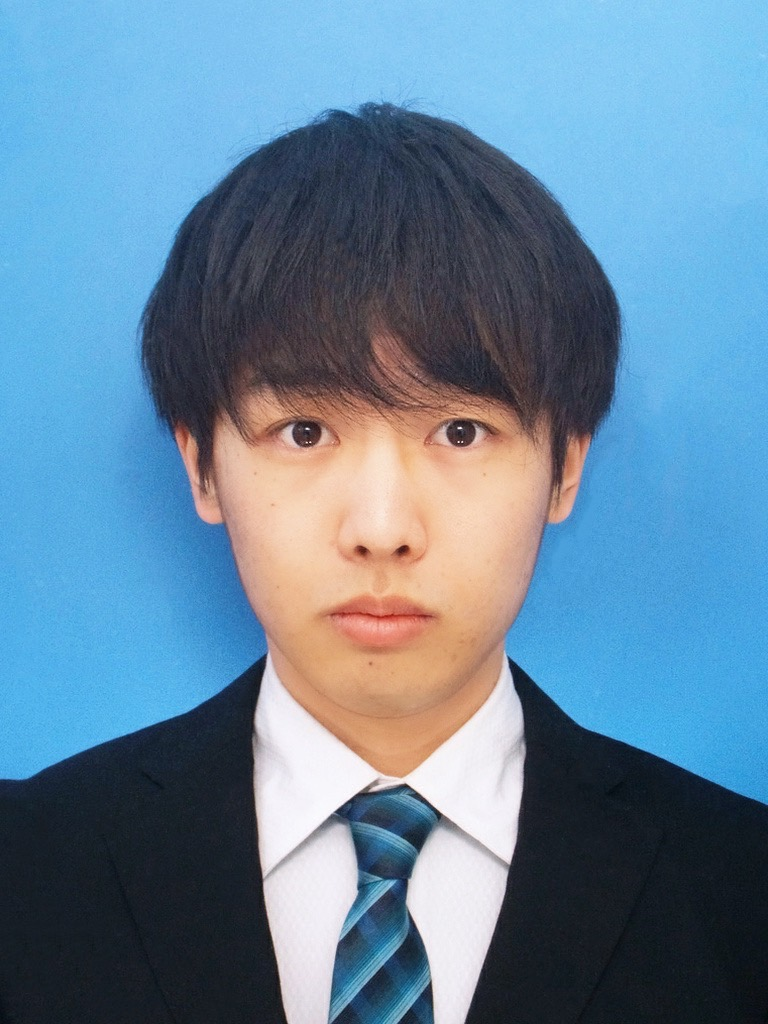
\includegraphics[width=1in,height=1.25in,clip,keepaspectratio]{author1.jpg}}]{Shogo Shimada} received the B.S. degree in computer science from Tokyo Metropolitan University in 2022. He is currently a Master's student at the Department of Computer Science, Graduate School of Systems Design, Tokyo Metropolitan University. His research interests include virtual reality, machine learning, deep learning, and human-computer interaction. He is a member of ACM.
\end{IEEEbiography}

\begin{IEEEbiography}[{
\includegraphics[width=1in,height=1.25in,clip,keepaspectratio]{author2.jpg}}]{Peerawat Pannattee} received his B.E. degree in electronics and telecommunication engineering and his M.E. degree in electrical engineering from King Mongkut’s University of Technology Thonburi (KMUTT), Bangkok, Thailand, in 2019 and 2022, respectively. Currently, he is pursuing his Ph.D. in computer science at Tokyo Metropolitan University in Tokyo, Japan. His research interests include image processing, computer vision, machine learning, deep learning, virtual reality, and human-computer interaction.
\end{IEEEbiography}

\begin{IEEEbiography}[{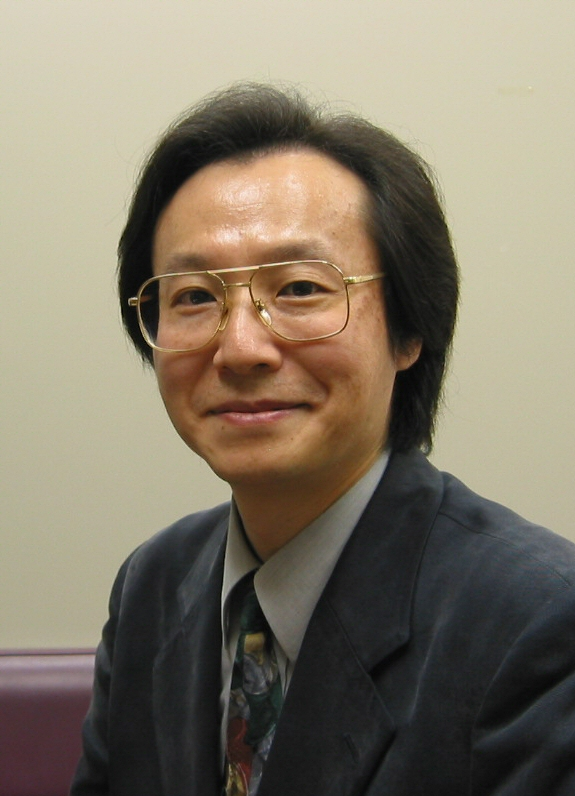
\includegraphics[width=1in,height=1.25in,clip,keepaspectratio]{author3.jpg}}]{Yasushi Ikei} received a Ph.D. degree in the industrial mechanical engineering from the University of Tokyo in 1988. He joined Tokyo Metropolitan Institute of Technology in 1992. After he worked for Tokyo Metropolitan University as Professor, he moved to the University of Tokyo. He is currently Professor at the Graduate School of Information Science and Technology, and Professor Emeritus at Tokyo Metropolitan University. His research interests are in the areas of virtual reality, ultra reality, telepresence, multisensory display, and cognitive engineering. He is a member of ACM, IEEE, JSME, and a fellow and former vice president of the VRSJ (Virtual Reality Society of Japan).
\end{IEEEbiography}

\begin{IEEEbiography}[{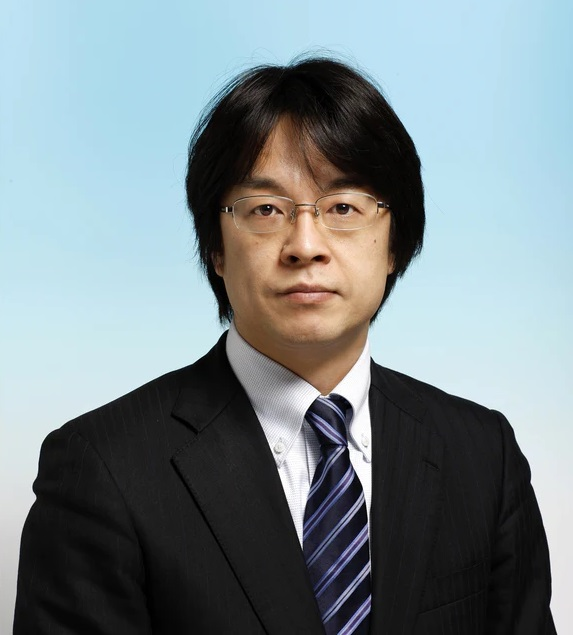
\includegraphics[width=1in,height=1.25in,clip,keepaspectratio]{author4.jpg}}]{Nobuyuki Nishiuchi} received his Ph.D. degree in engineering from Yokohama National University, Japan, in 2004. He is currently a Professor at Faculty of Systems Design, Tokyo Metropolitan University. His main research fields are human interface, usability engineering, image processing, ergonomics and biometrics. He is a member of IEEE, and served as a member of the International Program Committee for international conferences such as ICBAKE and CISIM for several times.
\end{IEEEbiography}

% \vspace{-32\baselineskip}

\begin{IEEEbiography}[{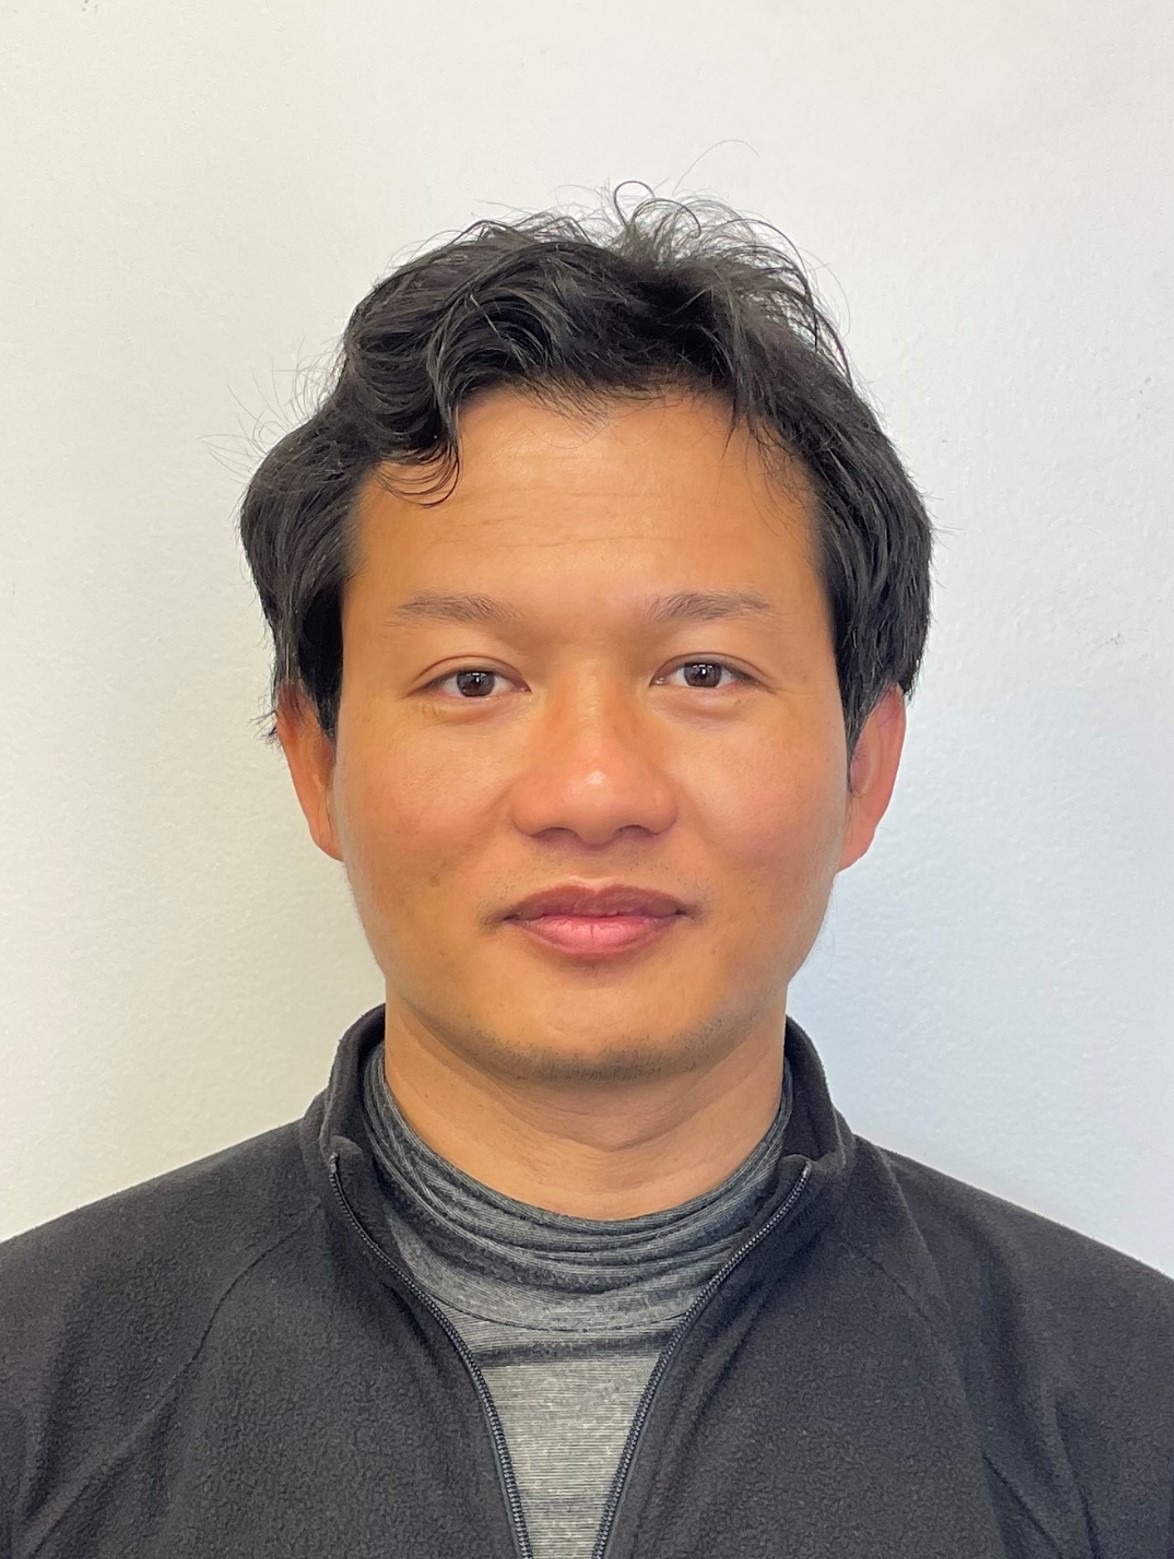
\includegraphics[width=1in,height=1.25in,clip,keepaspectratio]{author5.jpg}}]{Vibol Yem} received a Ph.D. in engineering from the University of Tsukuba in 2015. He is currently an associate professor at the  Faculty of  Engineering, Information and Systems, University of Tsukuba. He was an assistant professor at Tokyo Metropolitan Unversity from Apr 2018 to Feb 2023. His research interests are Human Interface, Tactile/Haptic Device, VR/AR, Wearable, Robotics. He is a member of ACM and IEEE Computer Society.
\end{IEEEbiography}

\EOD

\end{document}
